
\chapter {Theoretical Background}
\label{ch:TheoreticalBackground}

This chapter provides the theoretical foundation for the key concepts relevant to the design and implementation of this project. It focuses on topics related to Large Language Models (LLMs) and the architectural characteristics of Apple Silicon (M1/M2). The sections that follow explore essential components of LLM inference, the unique hardware features of Apple Silicon, and optimizations leveraged to enable efficient on-device performance.

%----------------------
\subsection{Large Language Models and Inference Components}
\label{sec:LargeLanguageModelsAndInferenceComponents} 
%----------------------

Large Language Models (LLMs) are transformer-based neural networks trained on massive text corpora to generate text in human language. They can mimic human-like conversations, storytelling, and can respond to abstract instructions. These models, such as GPT, LLaMA, and Falcon, rely on the transformer architecture introduced by Vaswani et al.~\cite{vaswani2017attention}, where self-attention mechanisms enable the model to capture dependencies across different parts of the input sequence (as seen in Figure ~\ref{fig:transformer_architecture}). Inference in LLMs involves several critical components, each contributing to performance, quality, and resource efficiency.

\begin{figure}[h]
    \centering
    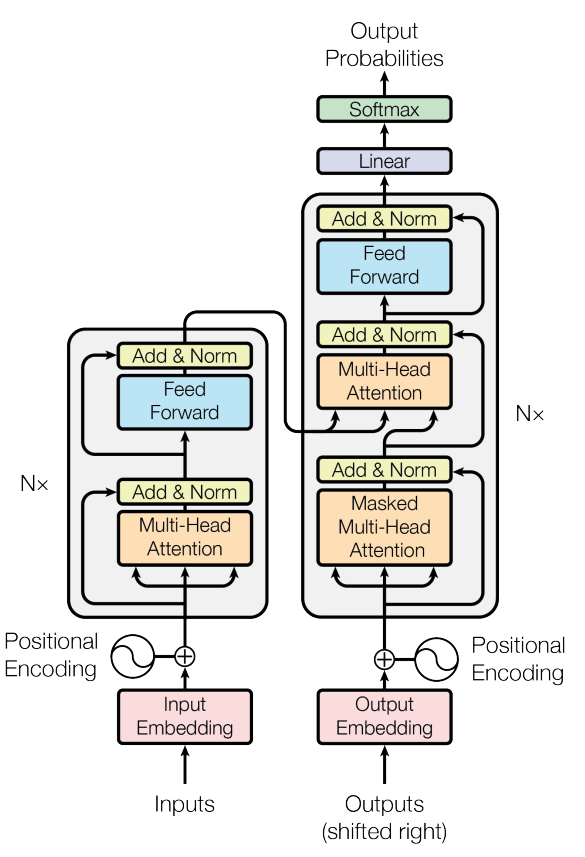
\includegraphics[width=0.4\linewidth]{images/transformer-architecture.png}
    \caption{Transformer architecture ~\cite{vaswani2017attention}}
    \label{fig:transformer_architecture}
\end{figure}
At the core of LLM inference lies the \textbf{context window}, which denotes the maximum number of tokens the model can attend to at any given time. A token is a piece of input, ranging from a subword to even a phrase, depending on the tokenization scheme of the model. For models like LLaMA-2, the context window can be up to 4,096 or 8,192 tokens~\cite{touvron2023llama}. During inference, the model builds an internal representation of this input context, which is used to generate predictions for the next token.

\begin{figure}[h]
    \centering
    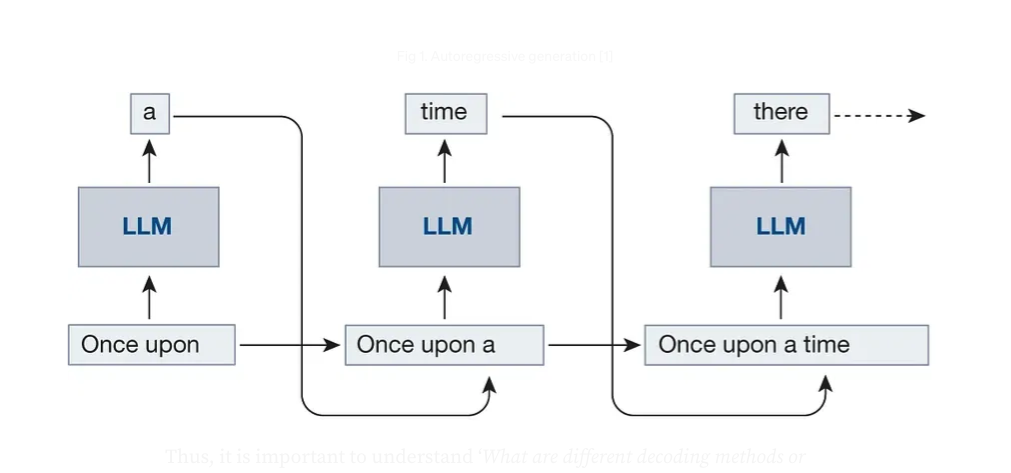
\includegraphics[width=0.6\linewidth]{images/autoregressive-decoding.png}
    \caption{Autoregressive decoding ~\cite{nabi2024all}}
    \label{fig:autoregressive_decoding}
\end{figure}

The \textbf{Key-Value (KV) cache} is a performance optimization central to LLM performance. During autoregressive decoding for text generation, a Large Language Model (LLM) processes the entire input sequence to generate a single output token. This newly generated token is then appended to the sequence, and the model repeats the process iteratively (as seen in Figure ~\ref{fig:autoregressive_decoding}). However, this leads to redundant computation over previously processed tokens at each step. To mitigate this inefficiency, the \textit{key} and \textit{value} vectors computed during the attention mechanism of the transformer can be cached. This \textit{KV caching} technique significantly reduces repeated computation by reusing the stored attention states from prior steps, thereby improving inference speed and memory efficiency. These cached representations allow the model to efficiently attend to all previously generated tokens without recalculating the entire attention graph ~\cite{alammar2018illustrated}. This caching mechanism reduces computational overhead and is especially vital when running LLMs on resource-constrained devices.

Furthermore, the token generation is governed by a sampling algorithm, which yields the output token by sampling on the output probability distribution obtained from the model. Common strategies include greedy sampling, top-$k$ sampling and temperature scaling. A \textbf{token sampler} module is responsible for leveraging these strategies to generate the output token. This can be a resource-hungry step, since this involves processing the probability distribution over the entire vocabulary of the model.

Therefore, the core components required for consistent text generation in an LLM-based system include the model weights, the LLM context (comprising the KV cache and vocabulary), and the token sampler.

Finally, the inference engine managing the model (e.g., llama.cpp, Hugging Face Transformers, or Apple CoreML) orchestrates the context construction, efficient memory handling of the KV cache, and optimized computation for each transformer layer, accounting for quantization if any. These components together define the responsiveness, accuracy, and resource efficiency of the LLM in real-time applications.

%----------------------
\subsection{LLM Weight Quantization}
\label{sec:LLMWeightQuantization} 
%----------------------
Quantization is a model weight compression technique that reduces the precision of the numbers used for representing model parameters. Typically, reducing the precision from 32-bit floating point to lower-bit integers such as 8-bit, 4-bit, or even 3-bit values. This significantly decreases memory usage and computational requirements, making it possible to run large language models (LLMs) efficiently on edge devices or in real-time environments without sacrificing too much accuracy \cite{jacob2017quantization,hubara2016quantized}.

Within the \texttt{ggml} framework and its application in \texttt{llama.cpp} \cite{llamacpp2023}, various quantization schemes have been introduced to significantly reduce the size and memory footprint of LLM weights. One such scheme is \texttt{Q3\_K\_L}, a 3-bit quantization format specifically designed to balance compression efficiency and model performance \cite{talamdupula2024guide,li2024quantization}. In \texttt{Q3\_K\_L}, weights are grouped in sets of 256 and quantized with shared scaling factors, offset by a zero-point, enabling fine-grained approximation while preserving hardware efficiency. Notably, \texttt{Q3\_K\_L} makes use of 4-bit storage for each quantized value (3 bits for the quantized magnitude and 1 extra bit for improved alignment and bit-packing efficiency), along with 8-bit scales and 6-bit zero-points per group. This layout ensures better alignment with SIMD instructions and allows for faster matrix-vector multiplications, which are critical during transformer inference \cite{pope2022efficiently}. ~\ref{tab:quantization-comparison} shows the comparison between common quantization schemes used in GGML. While this format slightly increases decoding complexity compared to simpler formats like \texttt{Q4\_0}, it provides a favorable tradeoff between model accuracy and size, especially for models deployed in edge or offline settings \cite{ollama2023,llamafile2023}.
Therefore, this project primarily employs model weights quantized using the \texttt{Q3\_K\_L} scheme.

\begin{table}[h]
\centering
\caption{Comparison of Common Quantization Formats in \texttt{ggml}/\texttt{llama.cpp}}
\label{tab:quantization-comparison}
\begin{tabular}{|l|c|c|c|c|}
\hline
\textbf{Format} & \textbf{Bits/Weight} & \textbf{Group Size} & \textbf{Remarks} \\ \hline
Q4\_0     & 4 bits   & 32 weights          & Baseline 4-bit scheme \\ \hline
Q4\_K     & 4 bits   & 64 weights    & Better accuracy than Q4\_0 \\ \hline
Q5\_K     & 5 bits   & 64 weights           & Higher accuracy, more storage \\ \hline
Q8\_0     & 8 bits   & 1 weight                          & No compression, baseline FP8 \\ \hline
\textbf{Q3\_K\_L}  & 3.5 bits avg & 256 weights  & High compression, optimized for SIMD \\ \hline
\end{tabular}
\end{table}
%----------------------
\section{Direct Numerical Simulations, RANS and LES}
\label{sec:DirectNumericalSimulationsRANSAndLES} 
%----------------------

In computational fluid dynamics (CFD), Direct Numerical Simulation (DNS), Reynolds-Averaged Navier-Stokes (RANS), and Large Eddy Simulation (LES) are three common approaches for simulating fluid flows, each with its own set of advantages and limitations.

DNS directly solves the Navier-Stokes equations without any modeling assumptions, providing detailed information on all scales of motion in the flow. However, DNS requires high computational resources and is typically only feasible for relatively low Reynolds number flows due to its high computational cost scaling with the cube of the Reynolds number.

RANS averages the Navier-Stokes equations over time to obtain mean flow quantities and then models the effects of turbulent fluctuations using empirical turbulence models. RANS is computationally less expensive than DNS and is suitable for a wide range of engineering applications. However, RANS relies on turbulence models that introduce modeling errors and uncertainties, particularly for complex flows.

LES resolves large-scale turbulent structures explicitly while modeling the effects of smaller-scale turbulence. It strikes a balance between the accuracy of DNS and the computational cost of RANS, making it suitable for simulating moderately high Reynolds number flows. LES captures the essential features of turbulence while reducing modeling errors compared to RANS.

\begin{figure}[H]
    \centering
    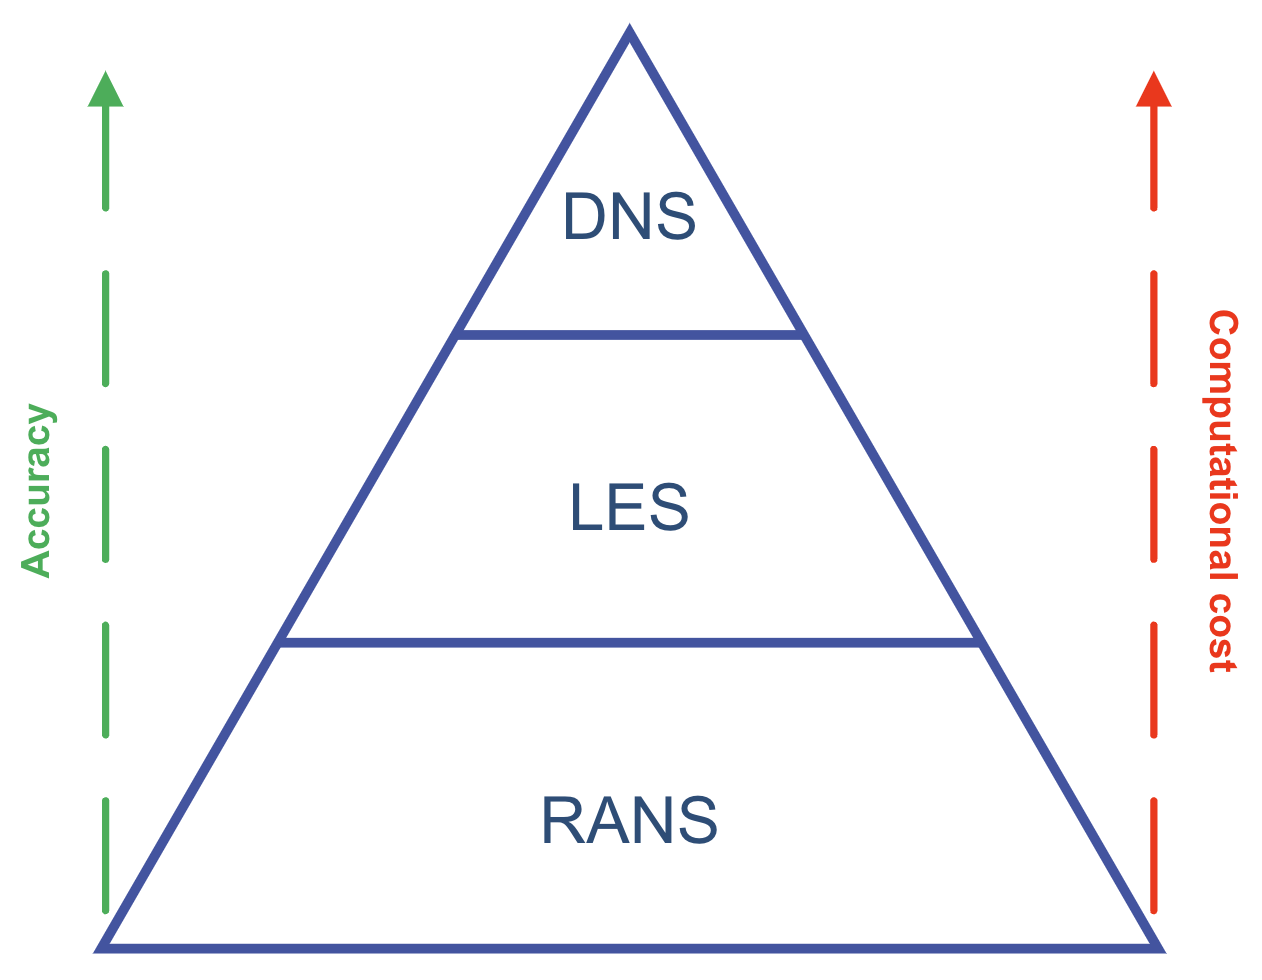
\includegraphics[width=0.4\linewidth]{images/dns_les_rans.png}
    \caption{Comparison between DNS, LES, and RANS modeling}
    \label{fig:dns_les_rans}
\end{figure}

The choice between DNS, RANS, and LES depends on the flow's specific characteristics, the desired detail level, and the available computational resources. Figure~\ref{fig:dns_les_rans} shows a comparison between the different modeling approaches. DNS provides the most accurate results but is computationally expensive, while RANS and LES offer compromises between accuracy and computational cost, making them more practical for many engineering applications.

%----------------------
\section{Time series}
\label{sec:TimeSeries} 
%----------------------

Time Series is a type of data that presents a temporal ordering. It is used in many real-world applications, such as signal processing, finance, weather forecasting, control engineering, communication, human activity recognition, cyber-security, or earthquake prediction. Time series can be described as univariate or multidimensional. Univariate or 1-dimensional time series is an ordered set of real values $X$ of length equal to the number of real values $T$, where $X = [x_1, x_2, ..., x_T]$. While a multidimensional or M-dimensional time series consists of M different univariate time series, where $X = [X^1, X^2, ..., X^M]$ with $X^i \in \mathbb{R}^T$. A Time Series Dataset is defined as $D = \{(X_1, Y_1), (X_2, Y_2), ..., (X_N, Y_N)\}$ as a collection of pairs $(X_i, Y_i)$ where $X_i$ could be a 1-dimensional or M-dimensional time series and an output $Y_i$.

%----------------------
\section{LSTM}
\label{sec:LSTM} 
%----------------------

Recurrent Neural Networks (RNN) are a type of neural network that can keep information about what happened before, they do this with loop connections to their neurons. These neural networks are widely used in speech recognition, language modeling, translation, etc. The main problem with this simple architecture is with “long-term dependencies” when the relevant information happened too long ago. Long Short Term Memory (LSTM) networks are designed to learn long-term dependencies to overcome this issue. The main idea behind the LSTM structure is a memory cell that can accumulate information that can be written and cleared by structures called gates. Fully Connected LSTM (FC-LSTM) is a multivariate version of LSTM, meaning that the input, output, and state are all 1-dimensional vectors.

LSTM neural networks are widely used in Natural Language Processing (NLP), where a long sequence of words in a text needs to be analyzed and used for prediction and classification.

%----------------------
\section{Convolutional Neural Networks}
\label{sec:CNN}
%----------------------

Convolutional Neural Networks (CNN) are a type of neural network primarily designed to process and analyze data in a grid-like organization, especially visual data such as images. Inspired by the organization of the animal visual cortex in the brain, CNNs have been successful in computer vision applications. The key operation in CNNs is the convolution mathematical operation, a specialized kind of linear operation. These networks have a structure called filters, which are applied to the input data to extract features, allowing the neural network to learn hierarchical representations.

CNNs have become the cornerstone of various computer vision tasks, including image classification, object detection, facial recognition, and medical image analysis. Their ability to automatically learn relevant features from raw data makes them particularly effective in tasks where traditional algorithms struggle, such as image understanding and pattern recognition. Additionally, CNNs offer advantages such as parameter sharing, which reduces the number of parameters and enhances model efficiency and translational invariance, enabling robust performance even with variations in object position within an image. Overall, CNNs have revolutionized the field of computer vision and continue to drive advancements in artificial intelligence and image processing applications.

%----------------------
\section{ConvLSTM}
\label{sec:ConvLSTM} 
%----------------------

LSTM neural networks are good for long-time series prediction because they are designed to maintain a context memory of important information that happened long ago as well as recent information. In applications with many dimensions, like spatial data, using an LSTM is inefficient as it contains too much redundancy in the connections between the input. 

ConvLSTM extends the Long Short-Term Memory (LSTM) architecture, incorporating convolutional operations within the LSTM units. It is specifically designed to handle spatiotemporal data, such as video sequences or spatial-temporal patterns in data. ConvLSTM preserves the sequential memory capabilities of LSTM while exploiting the spatial information in data through convolutions. This allows it to capture both temporal dependencies and spatial correlations simultaneously, making it ideal for tasks like video prediction, precipitation nowcasting, and motion tracking. Compared to traditional LSTMs, ConvLSTMs excel in modeling spatial dependencies within sequences, enabling more accurate predictions and better handling of spatially structured data.

%----------------------
\section{Autoencoders}
\label{sec:Autoencoders} 
%----------------------

Autoencoders are an artificial neural network used for unsupervised learning tasks, particularly in dimensionality reduction and data compression. Comprising an encoder and a decoder, they aim to reconstruct input data while learning efficient representations. The encoder compresses the input into a lower-dimensional latent space, while the decoder reconstructs the original data from this representation. Advantages include their ability to learn meaningful representations from unlabeled data, aiding in feature extraction and data denoising. They are widely used in anomaly detection, image denoising, and data generation tasks. Additionally, autoencoders can serve as the foundation for generative models, such as variational autoencoders (VAEs) and generative adversarial networks (GANs), enabling the synthesis of new data samples. Their versatility, simplicity, and capability to learn compact representations make them valuable tools in various domains, including computer vision and natural language processing.

